% slides_dat.tex — Slide Beamer LaTeX cho phần thuyết trình của Đạt
% Biên dịch bằng XeLaTeX: xelatex slides_dat.tex

\documentclass[aspectratio=169,10pt]{beamer}
\usetheme{Madrid}
\usecolortheme{whale}

\usepackage{iftex}
\ifTUTeX
  \usepackage{fontspec}
  \IfFontExistsTF{Arial}{\setsansfont{Arial}}{}
\else
  \usepackage[utf8]{inputenc}
  \usepackage[T5]{fontenc}
\fi
\usepackage{booktabs}
\usepackage{graphicx}

\title[NER Tiếng Việt trên PhoNER\_COVID19]{Nhận dạng Thực thể Có tên (NER) Tiếng Việt trên \texttt{PhoNER\_COVID19}}
\subtitle{Phần trình bày của Đạt: Bài toán, Dữ liệu \& EDA, Hợp đồng Đánh giá, Phân tích lỗi \& Demo}
\author[Đạt, Tín, Đức Anh]{Đạt \and Tín \and Đức Anh}
\institute[UET-VNU]{Khoa Công nghệ Thông tin — Trường Đại học Công nghệ, ĐHQGHN}
\date{Học kỳ I, 2026}

\begin{document}

\begin{frame}
  \titlepage
\end{frame}

\begin{frame}{1. Phát biểu Bài toán \& Thách thức trên Miền Y tế Tiếng Việt}
  \begin{itemize}
    \item \textbf{Đầu vào:} Câu tiếng Việt gồm $N$ token $\mathbf{x} = (x_1, \dots, x_N)$ ở mức từ (\texttt{word-level}, âm tiết trong từ ghép nối bằng \texttt{``\_''}) hoặc mức âm tiết (\texttt{syllable-level}).
    \item \textbf{Đầu ra:} Chuỗi $N$ nhãn BIO $\hat{\mathbf{y}} \in \mathcal{Y}^N$ ($21$ nhãn cố định: \texttt{O} + \texttt{B-/I-} của $10$ loại thực thể) $\rightarrow$ tập thực thể $\{(c_k, s_k, e_k)\}$.
    \item \textbf{3 thách thức cốt lõi:}
      \begin{enumerate}
        \item \textbf{Ranh giới từ ghép:} Khoảng trắng trong tiếng Việt tách âm tiết chứ không tách từ.
        \item \textbf{Tỉ lệ OOV cao ở thực thể định danh mới:} Mã bệnh nhân (\texttt{BN1347}), tên viết tắt (\texttt{N.H.N.}), số hiệu chuyến bay (\texttt{VN0054}).
        \item \textbf{Nhập nhằng vai trò ngữ cảnh:} Cùng cụm \texttt{``Bệnh\_viện Đà\_Nẵng''} có thể là \texttt{LOCATION} hoặc \texttt{ORGANIZATION}.
      \end{enumerate}
  \end{itemize}
\end{frame}

\begin{frame}{2. Thống kê Bộ dữ liệu \texttt{PhoNER\_COVID19} (Từ Notebook EDA)}
  \begin{table}
    \centering
    \footnotesize
    \begin{tabular}{lrrrrrr}
      \toprule
      \textbf{Tập} & \textbf{Số câu} & \textbf{Số từ (Word)} & \textbf{Số âm tiết} & \textbf{Dài TB (từ)} & \textbf{Thực thể} & \textbf{Tỉ lệ \texttt{O}} \\
      \midrule
      \texttt{train} & $5.027$ & $132.511$ & $167.541$ & $26{,}36$ & $15.767$ & $79{,}05\%$ \\
      \texttt{dev}   & $2.000$ & $56.283$  & $71.325$  & $28{,}14$ & $7.478$  & $74{,}92\%$ \\
      \texttt{test}  & $3.000$ & $85.678$  & $108.354$ & $28{,}56$ & $11.735$ & $74{,}17\%$ \\
      \midrule
      \textbf{Tổng}  & $\mathbf{10.027}$ & $\mathbf{274.472}$ & $\mathbf{347.220}$ & $\mathbf{27{,}37}$ & $\mathbf{34.980}$ & $\mathbf{76{,}68\%}$ \\
      \bottomrule
    \end{tabular}
  \end{table}
  \begin{itemize}
    \item \textbf{Mất cân bằng lớp mạnh:} \texttt{LOCATION} ($35{,}95\%$) và \texttt{PATIENT\_ID} ($18{,}64\%$) chiếm hơn một nửa; trong khi \texttt{JOB} ($1{,}46\%$) và \texttt{TRANSPORTATION} ($1{,}45\%$) rất hiếm.
    \item \textbf{Tỉ lệ OOV trên \texttt{test} so với từ điển \texttt{train} ($5.169$ từ):} Toàn tập chỉ $2{,}96\%$, nhưng riêng token thuộc \texttt{NAME} là $\mathbf{38{,}4\%}$, \texttt{TRANSPORTATION} là $\mathbf{34{,}7\%}$, \texttt{PATIENT\_ID} là $\mathbf{14{,}7\%}$.
  \end{itemize}
\end{frame}

\begin{frame}{3. Pipeline Dữ liệu, Từ điển \& Hợp đồng Batch (\texttt{src/data/})}
  \begin{itemize}
    \item \textbf{21 nhãn BIO cố định (\texttt{labels.py}):} \texttt{O} có \texttt{id = 0}; $10$ loại xếp theo bảng chữ cái để mọi thành viên dùng chung một \texttt{LABEL2ID}.
    \item \textbf{Từ điển chỉ xây từ \texttt{train} (\texttt{vocab.py}):}
      \begin{itemize}
        \item Ngăn rò rỉ dữ liệu (\textit{data leakage}) từ \texttt{dev/test}.
        \item Ngưỡng \texttt{min\_freq} đưa từ hiếm về \texttt{<unk>} (id=1) để mô hình học được vector biểu diễn cho từ lạ.
      \end{itemize}
    \item \textbf{Hợp đồng Batch cho BiLSTM-CRF (\texttt{bilstm\_dataset.py}):}
      \begin{itemize}
        \item \texttt{word\_ids [B, L]}, \texttt{char\_ids [B, L, W]}, \texttt{mask [B, L]} (\texttt{bool}), \texttt{tags [B, L]} (\texttt{long}), \texttt{lengths [B]}.
        \item Đệm \texttt{tags} bằng $0$ (\texttt{O}) thay vì $-100$ để tầng CRF \texttt{gather} hợp lệ rồi nhân \texttt{mask}.
      \end{itemize}
  \end{itemize}
\end{frame}

\begin{frame}{4. Thước đo Đánh giá \& Phân tích Lỗi 4 Nhóm (\texttt{src/evaluation/})}
  \begin{itemize}
    \item \textbf{Chấm điểm mức thực thể nghiêm ngặt (\texttt{metrics.py}):}
      \begin{itemize}
        \item Quy mọi dự đoán về đúng độ dài câu mức từ gốc $\text{len}(\text{\texttt{words}})$.
        \item Dùng \texttt{seqeval} (\texttt{mode="strict", scheme=IOB2}): chỉ tính đúng khi khớp cả ranh giới đầu--cuối lẫn loại thực thể; phạt các chuỗi bắt đầu bằng \texttt{I-X} mồ côi.
      \end{itemize}
    \item \textbf{Phân rã 4 nhóm lỗi loại trừ lẫn nhau (\texttt{error\_analysis.py}):}
      \begin{enumerate}
        \item \textbf{Boundary:} Đúng loại nhưng lệch ranh giới (hay gặp ở \texttt{ORGANIZATION}, \texttt{LOCATION} dài).
        \item \textbf{Type:} Giao nhau nhưng nhầm loại (\texttt{LOCATION} $\leftrightarrow$ \texttt{ORGANIZATION}).
        \item \textbf{False Positive (FP):} Báo nhầm thực thể trên vùng nhãn \texttt{O}.
        \item \textbf{False Negative (FN):} Bỏ sót hoàn toàn thực thể chuẩn.
      \end{enumerate}
    \item \textbf{Bảng kết quả chính:} \texttt{BiLSTM-CRF} đạt \texttt{[CHỜ SỐ LIỆU: Micro-F1 BiLSTM-CRF]}\% vs. \texttt{PhoBERT} đạt \texttt{[CHỜ SỐ LIỆU: Micro-F1 PhoBERT]}\%.
  \end{itemize}
\end{frame}

\begin{frame}{5. Trực quan hóa Thang xám \& Ứng dụng Demo Gradio (\texttt{app/})}
  \begin{columns}
    \begin{column}{0.52\textwidth}
      \begin{itemize}
        \item \textbf{Hình vẽ chuẩn ACL (đọc rõ ở thang xám):}
          \begin{itemize}
            \item Kết hợp độ đậm xám + hoa văn gạch chéo (\textit{hatch}).
            \item Xuất tự động vector \texttt{.pdf} từ \texttt{01\_eda} và \texttt{04\_error\_analysis}.
          \end{itemize}
        \item \textbf{Demo Gradio (\texttt{python -m app.demo}):}
          \begin{itemize}
            \item Tự động tách từ bằng \texttt{Underthesea}.
            \item Hàm cắm \texttt{load\_model(path)} hỗ trợ nạp checkpoint của cả Tín và Đức Anh hoặc chạy chế độ \texttt{dummy}.
          \end{itemize}
      \end{itemize}
    \end{column}
    \begin{column}{0.46\textwidth}
      \centering
      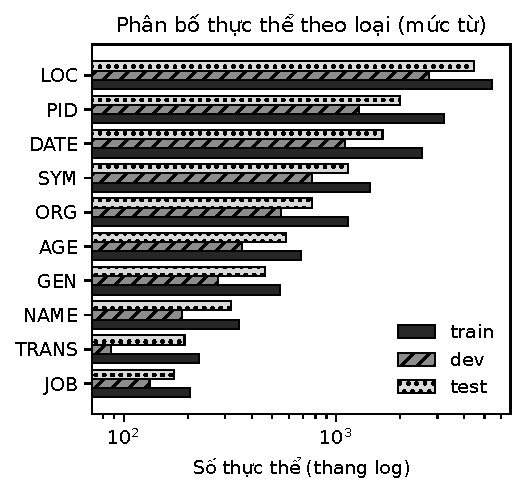
\includegraphics[width=0.95\textwidth]{../outputs/figures/eda_entity_distribution.pdf}
    \end{column}
  \end{columns}
\end{frame}

\end{document}
